
{\parindent0pt
\fbox{\begin{minipage}{0.96\textwidth}
Gunnar Wolf, Esteban Ruiz, Federico Bergero, Erwin Meza
\\
\\Sistemas Operativos

1a ed. - Iniciativa Latinoamericana de Libros de Texto Abiertos (LATIn), 2014. 247 pag.
\end{minipage}}

\vspace{2em}

Primera Edici\'on: Marzo 2014

Iniciativa Latinoamericana de Libros de Texto Abiertos (LATIn)

\url{http://www.proyectolatin.org/}

\begin{figure}[h!]
    
\includegraphics[width=0.2\textwidth]{Pictures/creativecommons.png}
\end{figure}

Los textos de este libro se distribuyen bajo una licencia Reconocimiento-CompartirIgual 3.0 Unported (CC BY-SA 3.0) \url{http://creativecommons.org/licenses/by-sa/3.0/deed.es_ES}
\\
\\Esta licencia permite:

Compartir: copiar y redistribuir el material en cualquier medio o formato.

Adaptar: remezclar, transformar y crear a partir del material para cualquier finalidad.
\\
\\Siempre que se cumplan las siguientes condiciones:\\

\begin{wrapfigure}{l}{0.1\textwidth}
\vspace{-20pt}
  \begin{center}
    
\includegraphics[width=0.1\textwidth]{Pictures/by.jpg}
  \end{center}
\end{wrapfigure}
Reconocimiento. Debe reconocer adecuadamente la autor\'ia, proporcionar un enlace a la licencia e indicar si se han realizado cambios. Puede hacerlo de cualquier manera razonable, pero no de una manera que sugiera que tiene el apoyo del licenciador o lo recibe por el uso que hace.\\
\\

\begin{wrapfigure}{l}{0.1\textwidth}
\vspace{-32pt}
  \begin{center}
    
\includegraphics[width=0.1\textwidth]{Pictures/sa.jpg}
  \end{center}
\end{wrapfigure}
CompartirIgual -- Si remezcla, transforma o crea a partir del material, deber\'a difundir sus contribuciones bajo \underline{\textbf{la misma licencia que el original}}.
\\
\\Las figuras e ilustraciones que aparecen en el libro son de autor\'ia de los respectivos autores. De aquellas figuras o ilustraciones que no son realizadas por los autores, se coloca la referencia respectiva.

\begin{figure}[h!]
    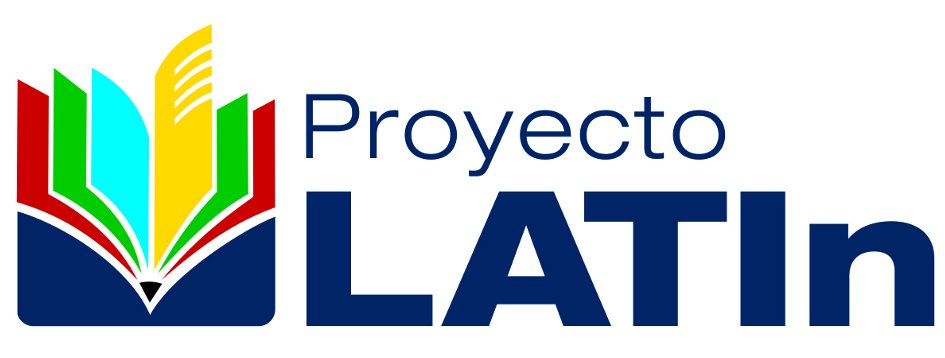
\includegraphics[width=0.2\textwidth]{Pictures/logolatin.jpg}
\end{figure}

Este texto forma parte de la Iniciativa Latinoamericana de Libros de Texto abiertos (LATIn), proyecto financiado por la Uni\'on Europea en el marco de su Programa ALFA III EuropeAid.\\
\\
El Proyecto LATIn est\'a conformado por: Escuela Superior Polit\'ecnica del Litoral, Ecuador (ESPOL); Universidad Aut\'onoma de Aguascalientes, Mexico (UAA), Universidad Cat\'olica de San Pablo, Per\'u (UCSP); Universidade Presbiteriana Mackenzie, Brasil(UPM); Universidad de la Rep\'ublica, Uruguay (UdelaR); Universidad Nacional de Rosario, Argentina(UR); Universidad Central de Venezuela, Venezuela (UCV), Universidad Austral de Chile, Chile (UACH), Universidad del Cauca, Colombia (UNICAUCA), Katholieke Universiteit Leuven, B\'elgica (KUL), Universidad de Alcal\'a, Espa\~na (UAH), Universit\'e Paul Sabatier, Francia (UPS).

}
